\section{Our Proposed Method for Bias Mitigation}
\label{mitigation_section}
\begin{figure*}[htb!]
  \centering
   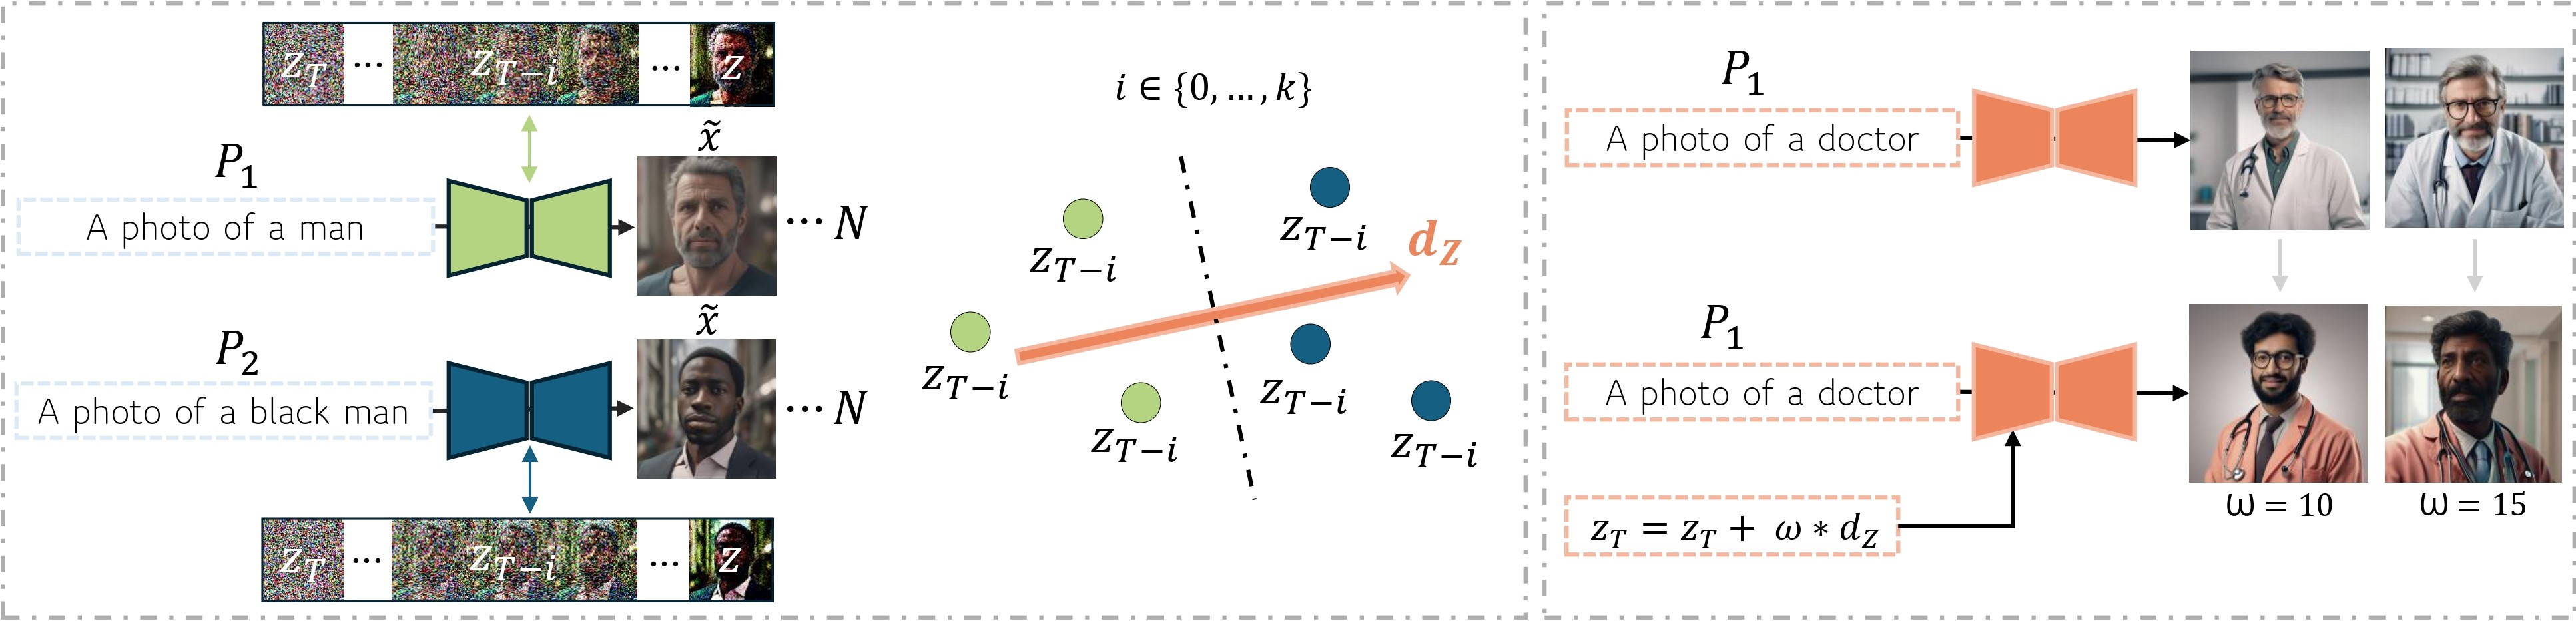
\includegraphics[width=1\linewidth]{images/method_paper_highQ.jpg}
  \caption{\textbf{Summary of our training (left) and inference (right) approach.} We use $P_{1}$ and $P_{2}$ to generate $N$ images $\Tilde{x}$. With their latents, chosen at step $i$, we train a $SVM$ to learn $d_{Z}$. We debias the neutral prompt $P_{1}$, applying $d_{Z}$ to the random initial latent $z_{T} \sim N(\mu, \sigma^2)$ at a specific $\omega$ weight, shifting the generations towards debiased samples with the attributes learned through the latent direction.}
  \label{fig:our_method_training_inference}
\end{figure*}
% Uncomment for a shorter option:
%Previous research in bias mitigation \cite{zhang2023itigen, chuang2023debiasing} focused on the alteration of prompt embeddings to condition the generations. However, given the image arises from the noise distribution [insert appendix], our approach learns the Gaussian Noise direction to condition the initial noise fed into the diffusion process, leaving the original neutral prompt and its embeddings left as is.
\noindent\textbf{Training: Finding the Latent Direction}
Our approach (Fig.~\ref{fig:our_method_training_inference}) proposes a fundamentally different transformation of the diffusion process's input, learning the latent direction $d_{Z}$, from the Gaussian latents at denoised steps, to condition the initial noisy information tensor fed into the diffusion process $z_{T} \sim \mathcal{N}(0, I)$. Given a pre-trained latent diffusion model (LDM) and a neutral prompt $P_{1}$ (\textit{e.g., "a photo of a man, in color, realistic, 8k"}), we aim to obtain debiased generations in the absence of prompt modifications or embeddings alterations. We propose a 'target' prompt $P_{2}$ (\textit{e.g., "a photo of a black man, in color, realistic, 8k"}) and sample $N$ number of images, for both $P_{1}$ and $P_{2}$, to construct the training dataset. The diffusion process for each of the prompts starts from an initial noisy latent  $z_{T}$, which is denoised over $k$ steps, finally reaching the ultimate latent $z$, fed into the decoder $D$ to generate the synthetic image $\tilde{x}$. 

While generating the $N$ images, we save each image's latents at chosen denoising steps $L = (L_{0}, \cdots, L_{k})$, representing ($z_{T},\cdots,z_{T-i}$ for $i \in \{0, 1, 2, \ldots, k\}$ ), building a dataset of noisy information tensors. Note, $L_{0}$ corresponds to the initial Gaussian latent $z_{T}$, while $L_{k}$ is $z$. Once all chosen latents are saved for both prompts, we select one denoising step $i$ to obtain $d_{Z}$ with those specific latents. For instance, we could decide to train with $L_{10}$, the latents saved for the $N$ images at step 10 ($z_{T-10}$). 

\noindent\textbf{The model.} We use a support vector machine (SVM) \cite{Vapnik2015} to linearly separate the latents across our labeled dataset of $N$ samples for each prompt. The classifier uses a linear kernel and provides the $d_{Z}$, the so-called \textit{latent direction}, we utilize for debiasing. 


\noindent\textbf{Inference: Applying the Latent Direction.}
To obtain debiased generations, the LDM, in our case Stable Diffusion \cite{rombach2022highresolution}, uses for inference only $P_{1}$, the neutral prompt. This prompt is fed into CLIP's text encoder $E$ forming the first input. As the second one, instead of using an initial Gaussian random information tensor for denoising, we transform this latent by applying the learned latent direction $d_{Z}$, following equation \ref{eq:important}. 

\begin{equation}
  z_{T} = z_{T} + \omega \cdot d_{Z}
  \label{eq:important}
\end{equation}

Where $z_{T} \sim N(\mu, \sigma^2)$ and $\omega$ is the weight parameter at which the latent direction is applied. The higher the $\omega$, the higher the strength of the debiasing impact. 


%the other approaches inject the learned tokens or jiggle around these embeddings. 
% There is a tradeoffinvolved in finding the optimal latent to train the classifier. Out of 50 denoising steps

%We refer to this direction as \textit{latent direction} and to learn it, we utilize Stable Diffusion to generate two datasets of 50 samples each, using the neutral and the debiased prompt. The relevant part of these datasets are not the final generated images, but the noise latents involved in their denoising processes. In our case we have used 50 denoising steps, saving these latents every 5th step, obtaining 9 latents [L5, L10, L15 … L45] per image. For training, one of these latent steps is selected and fed as input data for a Support Vector Machine (SVM) classifier with a linear kernel.  The SVM provides two learned latent directions, the biased and debiased ones. As a result, to successfully mitigate biases we use the original neutral prompt, linearly combining the initial Gaussian noise with the weighted latent direction, following: 


\noindent\textbf{The optimal configuration.} Optimal debiasing results are found when selecting the most favorable latent $L = (L_{0}, \cdots, L_{k})$ and weight configuration $\omega$. Thus, we propose two approaches to automatically find it without having to visually explore all possibilities. The first one is to use the \textit{clean-fid} \cite{parmar2022aliased} library to compute the similarity between the distribution of a small subset of generated images with a particular configuration, and the distribution of known debiased images, and the second one is to leverage CLIP \cite{radford2021learning} as a zero-shot classifier, selecting the configuration with a high classification of the desired debiased class. 
%We find the effectivity of our method is conditioned upon the selection of the latent $L = (L_{0}, \cdots, L_{k})$ and weight configuration $\omega$, given each debiasing scenario has its own, and optimal debiasing results are achieved when found.
